\chapter{The SLAM problem}
\label{ch:slam}

A mower drives across the lawn. At each instant it knows two things: what
its wheels (or IMU) say it did since the last instant, and what its camera
sees now. It wants two things: where it is, and what the garden looks like.
Neither can be had without the other. To localise you need a map; to build
a map you need to know where you were when you saw each part of it. SLAM
solves both jointly. This chapter writes that joint problem down precisely,
shows that under Gaussian noise it is a nonlinear least-squares problem
whose structure is a sparse graph, and explains why modern visual SLAM
\emph{smooths} that graph instead of \emph{filtering} it, as your Kalman
and particle filters did.

\section{Variables, models and assumptions}

\begin{definition}{SLAM variables}{slamvars}
Over a discrete time horizon $k=0,\dots,K$ we consider
\begin{itemize}[nosep]
\item the \emph{states} (poses) $\x_k\in\mathcal{X}$ of the robot, collected
  in $X=\x_{0:K}$;
\item the \emph{landmarks} $\m_j\in\mathcal{M}$, $j=1,\dots,N$, collected
  in $M=\m_{1:N}$;
\item the \emph{controls} or proprioceptive measurements $\uu_k$,
  $k=1,\dots,K$ (wheel odometry, IMU), collected in $U$;
\item the \emph{observations} $\z_{kj}$, defined for the pairs $(k,j)$ in a
  set $\mathcal{O}$ of ``landmark $j$ seen at time $k$'', collected in $Z$.
\end{itemize}
The unknowns are $\btheta=(X,M)$. The data are $(U,Z)$.
\end{definition}

For a ground robot $\mathcal{X}$ is $\SE2$ or $\SE3$; for visual SLAM a
landmark is typically a 3D point, $\mathcal{M}=\R^3$. Chapter~\ref{ch:rigid}
treats the geometry of $\SE3$; for now the state space is abstract and,
where we need to subtract states, we pretend it is a vector space. The
whole point of Chapter~\ref{ch:rigid} is to make that pretence legitimate.

\begin{definition}{Motion and observation models}{models}
A \emph{motion model} and an \emph{observation model} are functions
\begin{align}
  \x_k &= f(\x_{k-1},\uu_k) + \vect{w}_k,
  & \vect{w}_k &\sim \Normal(\vect{0},\,Q_k),\label{eq:motion}\\
  \z_{kj} &= h(\x_k,\m_j) + \vect{v}_{kj},
  & \vect{v}_{kj} &\sim \Normal(\vect{0},\,R_{kj}),\label{eq:obs}
\end{align}
with all noises mutually independent and independent of the initial state
$\x_0\sim\Normal(\check{\x}_0,P_0)$.
\end{definition}

For a camera, $h$ is ``transform the point into the camera frame, then
project it on the image'' (Chapter~3), and $\z_{kj}\in\R^2$ is a pixel.

The two models encode two conditional-independence assumptions that are
worth naming, because every factorisation below rests on them.

\begin{definition}{Markov and measurement-independence assumptions}{markov}
\begin{enumerate}[label=(A\arabic*),nosep]
\item\label{A1} \emph{Markov motion}: given $\x_{k-1}$ and $\uu_k$, the
  state $\x_k$ is independent of all earlier states, controls and of the
  landmarks:
  $p(\x_k\mid \x_{0:k-1},\uu_{1:k},M)=p(\x_k\mid\x_{k-1},\uu_k)$.
\item\label{A2} \emph{Measurement independence}: given the states and the
  landmarks, the observations are mutually independent and each depends
  only on the pose and landmark involved, and on nothing in $U$:
  $p(Z\mid X,M,U)=\prod_{(k,j)\in\mathcal{O}}p(\z_{kj}\mid\x_k,\m_j)$.
\item\label{A3} \emph{Prior}: $p(\x_0,M)=p(\x_0)\,p(M)$, and the landmark
  prior $p(M)$ is either flat or itself factorised.
\end{enumerate}
\end{definition}

\section{The full posterior and its factorisation}

\begin{proposition}{Factorisation of the SLAM posterior}{factorisation}
Under \ref{A1}--\ref{A3},
\begin{equation}\label{eq:posterior}
  p(X,M\mid U,Z)\;\propto\;
  p(\x_0)\,p(M)
  \prod_{k=1}^{K}p(\x_k\mid\x_{k-1},\uu_k)
  \prod_{(k,j)\in\mathcal{O}}p(\z_{kj}\mid\x_k,\m_j).
\end{equation}
\end{proposition}

\begin{proof}
By Bayes' rule, conditioning everything on $U$,
\[
  p(X,M\mid U,Z)=\frac{p(Z\mid X,M,U)\,p(X,M\mid U)}{p(Z\mid U)}
  \propto p(Z\mid X,M,U)\,p(X,M\mid U),
\]
since the denominator does not depend on $(X,M)$. The first factor is the
product of observation likelihoods by \ref{A2}. For the second, the chain
rule gives
\[
  p(X,M\mid U)=p(\x_0,M\mid U)\prod_{k=1}^K
  p(\x_k\mid\x_{0:k-1},M,U).
\]
The initial pose and the landmarks do not depend on future controls, so
$p(\x_0,M\mid U)=p(\x_0,M)=p(\x_0)p(M)$ by \ref{A3}. In each remaining
factor, $\x_k$ does not depend on controls after time $k$ (the future does
not act on the past), and then \ref{A1} removes everything but
$\x_{k-1}$ and $\uu_k$. Multiplying the pieces gives \eqref{eq:posterior}.
\end{proof}

\begin{inwords}
The posterior over \emph{everything} is a product of small local pieces:
one per odometry step, one per pixel observation, one prior. Each piece
only ``touches'' the few variables it involves. This locality is the single
most important structural fact in SLAM: it is what makes problems with
thousands of poses and hundreds of thousands of points solvable in real
time.
\end{inwords}

\section{From MAP to nonlinear least squares}

We want a point estimate, the maximum a posteriori (MAP) estimate
$\btheta^\star=\arg\max_{\btheta}p(\btheta\mid U,Z)$. Write
$\norm{\vect{e}}_{\Sigma}^2=\vect{e}\T\Sigma^{-1}\vect{e}$ for the squared
Mahalanobis norm.

\begin{proposition}{MAP is weighted nonlinear least squares}{mapnls}
Under the Gaussian models of \cref{def:models}, a flat landmark prior and
\ref{A1}--\ref{A3},
\begin{equation}\label{eq:nls}
\btheta^\star=\arg\min_{\btheta}\;F(\btheta),\quad
F(\btheta)=\tfrac12\norm{\vect{e}_0}_{P_0}^2
 +\tfrac12\sum_{k=1}^{K}\norm{\vect{e}^{u}_k}_{Q_k}^2
 +\tfrac12\sum_{(k,j)\in\mathcal{O}}\norm{\vect{e}^{z}_{kj}}_{R_{kj}}^2,
\end{equation}
with residuals $\vect{e}_0=\x_0-\check\x_0$,
$\vect{e}^u_k=\x_k-f(\x_{k-1},\uu_k)$ and
$\vect{e}^z_{kj}=\z_{kj}-h(\x_k,\m_j)$.
\end{proposition}

\begin{proof}
The logarithm is strictly increasing, so maximising $p$ is minimising
$-\log p$. By \eqref{eq:motion}, $\x_k\mid\x_{k-1},\uu_k\sim
\Normal(f(\x_{k-1},\uu_k),Q_k)$, whose density is
$(2\pi)^{-n/2}\det(Q_k)^{-1/2}\exp(-\tfrac12\norm{\vect{e}^u_k}^2_{Q_k})$.
Its negative logarithm is $\tfrac12\norm{\vect{e}^u_k}^2_{Q_k}$ plus a
constant independent of $\btheta$ (the covariances are known). The same
holds for every observation term and for the prior on $\x_0$; the flat
landmark prior contributes a constant. Taking $-\log$ of
\eqref{eq:posterior} therefore gives $F(\btheta)$ plus a constant.
\end{proof}

\begin{inwords}
Each residual is ``what the model predicts versus what we measured'', and
each is divided by how much we trust that measurement. A pixel measured to
within half a pixel weighs a lot; a wheel odometry step on wet grass
weighs little. MAP estimation is just ``find the trajectory and map that
best explain all the evidence, each piece weighted by its reliability''.
\end{inwords}

It is convenient to whiten the residuals. If $\Sigma=LL\T$ is a Cholesky
factorisation, then $\norm{\vect{e}}_\Sigma^2=\norm{L^{-1}\vect{e}}^2$.
Stacking all whitened residuals into $\vect{r}(\btheta)$ gives the compact
form $F(\btheta)=\tfrac12\norm{\vect{r}(\btheta)}^2$, which is what every
solver in Chapter~4 minimises.

\section{Factor graphs}

\begin{definition}{Factor graph}{factorgraph}
A \emph{factor graph} is a bipartite graph $\mathcal{G}=(\mathcal{V}\cup
\mathcal{F},\mathcal{E})$ with \emph{variable nodes} $\mathcal{V}$ and
\emph{factor nodes} $\mathcal{F}$. Each factor $a\in\mathcal{F}$ is a
nonnegative function $\varphi_a(\btheta_a)$ of the variables
$\btheta_a$ it is connected to. The graph represents the function
\[
  \varphi(\btheta)=\prod_{a\in\mathcal{F}}\varphi_a(\btheta_a).
\]
For Gaussian factors, $\varphi_a(\btheta_a)=
\exp\bigl(-\tfrac12\norm{\vect{e}_a(\btheta_a)}^2_{\Sigma_a}\bigr)$, so that
$-\log\varphi=\sum_a\tfrac12\norm{\vect{e}_a}^2_{\Sigma_a}=F$.
\end{definition}

\Cref{prop:factorisation} says that the SLAM posterior \emph{is} a factor
graph, drawn in \cref{fig:fg}.

\begin{figure}[ht]
\centering
\begin{tikzpicture}[
  var/.style={circle,draw,thick,minimum size=8mm,inner sep=0pt},
  lm/.style={circle,draw,thick,fill=lawngreen!15,minimum size=8mm,
    inner sep=0pt},
  fac/.style={rectangle,fill=black,minimum size=2.2mm,inner sep=0pt},
  every edge/.style={draw,thick}]
\foreach \i in {0,...,3}{
  \node[var] (x\i) at (2.6*\i,0) {$\x_{\i}$};}
\node[lm] (m1) at (1.3,2.4) {$\m_1$};
\node[lm] (m2) at (5.2,2.4) {$\m_2$};
\node[lm] (m3) at (7.8,2.4) {$\m_3$};
\node[fac,label=left:{\small prior}] (p0) at (-1.1,0) {};
\draw[thick] (p0)--(x0);
\foreach \i [evaluate=\i as \j using int(\i+1)] in {0,1,2}{
  \node[fac,label=below:{\small$\uu_{\j}$}] (u\j) at (2.6*\i+1.3,0) {};
  \draw[thick] (x\i)--(u\j)--(x\j);}
\foreach \k/\j in {0/1,1/1,1/2,2/2,3/2,3/3}{
  \path (x\k) -- coordinate[pos=0.55] (c\k\j) (m\j);
  \node[fac] at (c\k\j) {};
  \draw[thick] (x\k)--(c\k\j)--(m\j);}
\end{tikzpicture}
\caption{The factor graph of a small SLAM problem. White nodes are poses,
green nodes landmarks, black squares factors: one prior, three odometry
factors and six observation factors.}
\label{fig:fg}
\end{figure}

\subsection{Sparsity of the normal equations}

All solvers of Chapter~4 iterate on a linear system
$H\,\delta\btheta=-\vect{g}$, with $H=J\T J$ the Gauss--Newton
approximation of the Hessian, $J=\partial\vect{r}/\partial\btheta$ and
$\vect{g}=J\T\vect{r}$. Partition $\btheta$ into blocks $\btheta_i$ (one
per pose, one per landmark) and $\vect{r}$ into blocks $\vect{r}_a$ (one
per factor).

\begin{proposition}{The factor graph is the sparsity pattern}{sparsity}
The block $H_{ij}$ can be nonzero only if variables $i$ and $j$ are both
connected to at least one common factor. In particular $H$ has the
sparsity pattern of the adjacency matrix of the graph obtained from the
factor graph by connecting any two variables that share a factor.
\end{proposition}

\begin{proof}
Since $\vect{r}$ is the stack of the $\vect{r}_a$,
$H=J\T J=\sum_{a}J_a\T J_a$, where $J_a=\partial\vect{r}_a/\partial\btheta$.
Thus $H_{ij}=\sum_a (J_{a,i})\T J_{a,j}$ with
$J_{a,i}=\partial\vect{r}_a/\partial\btheta_i$. The residual
$\vect{r}_a$ depends only on $\btheta_a$, so $J_{a,i}=0$ whenever
$\btheta_i\notin\btheta_a$. Each term of the sum is therefore zero unless
both $\btheta_i$ and $\btheta_j$ belong to $\btheta_a$.
\end{proof}

\begin{inwords}
In visual SLAM a pose sees a few hundred points, and a point is seen by a
handful of poses. So $H$ is overwhelmingly zero, with a very characteristic
``arrowhead'' structure that Chapter~8 exploits with the Schur complement.
\end{inwords}

\section{Filtering versus smoothing}

Your Kalman filters kept only the current state: at each step they
\emph{marginalised out} the previous one. EKF-SLAM does the same with the
state $(\x_k,M)$. The following lemma, which is also the heart of
sliding-window back-ends (Chapter~9), shows what marginalisation does to
the graph.

\begin{lemma}{Gaussian marginalisation in information form}{schur}
Let $(\x_a,\x_b)$ have density proportional to
$\exp\bigl(-\tfrac12\x\T\Lambda\x+\vect{\eta}\T\x\bigr)$ with
\[
  \Lambda=\begin{pmatrix}\Lambda_{aa}&\Lambda_{ab}\\
    \Lambda_{ba}&\Lambda_{bb}\end{pmatrix}\succ0,\qquad
  \vect{\eta}=\begin{pmatrix}\vect{\eta}_a\\\vect{\eta}_b\end{pmatrix}.
\]
Then the marginal of $\x_a$ is proportional to
$\exp\bigl(-\tfrac12\x_a\T\Lambda'\x_a+\vect{\eta}'^{\mathsf T}\x_a\bigr)$
with
\begin{equation}\label{eq:schur}
\Lambda'=\Lambda_{aa}-\Lambda_{ab}\Lambda_{bb}^{-1}\Lambda_{ba},\qquad
\vect{\eta}'=\vect{\eta}_a-\Lambda_{ab}\Lambda_{bb}^{-1}\vect{\eta}_b .
\end{equation}
$\Lambda'$ is the Schur complement of $\Lambda_{bb}$ in $\Lambda$.
\end{lemma}

\begin{proof}
Since $\Lambda$ is symmetric, $\Lambda_{ba}=\Lambda_{ab}\T$. The exponent is
\[
\Phi=-\tfrac12\x_a\T\Lambda_{aa}\x_a-\x_a\T\Lambda_{ab}\x_b
-\tfrac12\x_b\T\Lambda_{bb}\x_b+\vect{\eta}_a\T\x_a+\vect{\eta}_b\T\x_b .
\]
Collect the terms in $\x_b$: $-\tfrac12\x_b\T\Lambda_{bb}\x_b
+\x_b\T\vect{c}$ with $\vect{c}=\vect{\eta}_b-\Lambda_{ba}\x_a$.
$\Lambda_{bb}\succ0$ (a principal block of a positive definite matrix), so
we may complete the square with $\vect{\mu}=\Lambda_{bb}^{-1}\vect{c}$:
\[
-\tfrac12\x_b\T\Lambda_{bb}\x_b+\x_b\T\vect{c}
=-\tfrac12(\x_b-\vect{\mu})\T\Lambda_{bb}(\x_b-\vect{\mu})
+\tfrac12\vect{c}\T\Lambda_{bb}^{-1}\vect{c}.
\]
Integrating $\exp$ of the first term over $\x_b$ gives
$(2\pi)^{n_b/2}\det(\Lambda_{bb})^{-1/2}$, which does not depend on
$\x_a$. What remains in the exponent is
\begin{align*}
&-\tfrac12\x_a\T\Lambda_{aa}\x_a+\vect{\eta}_a\T\x_a
+\tfrac12(\vect{\eta}_b-\Lambda_{ba}\x_a)\T\Lambda_{bb}^{-1}
  (\vect{\eta}_b-\Lambda_{ba}\x_a)\\
&=-\tfrac12\x_a\T\bigl(\Lambda_{aa}-\Lambda_{ab}\Lambda_{bb}^{-1}
  \Lambda_{ba}\bigr)\x_a
 +\bigl(\vect{\eta}_a-\Lambda_{ab}\Lambda_{bb}^{-1}\vect{\eta}_b\bigr)\T
  \x_a+\text{const},
\end{align*}
where we expanded the quadratic and used
$(\Lambda_{ba}\x_a)\T\Lambda_{bb}^{-1}\vect{\eta}_b
=\x_a\T\Lambda_{ab}\Lambda_{bb}^{-1}\vect{\eta}_b$.
\end{proof}

\begin{proposition}{Marginalisation creates fill-in}{fillin}
Marginalising a variable $\x_b$ out of a Gaussian factor graph produces a
new information matrix in which every pair of variables that were
neighbours of $\x_b$ becomes connected.
\end{proposition}

\begin{proof}
By \cref{prop:sparsity} the block $\Lambda_{ib}$ is nonzero only for
neighbours $i$ of $\x_b$. The correction term in \eqref{eq:schur} has
blocks $\Lambda_{ib}\Lambda_{bb}^{-1}\Lambda_{bj}$, generically nonzero
whenever both $i$ and $j$ are neighbours of $\x_b$.
\end{proof}

\begin{inwords}
Forgetting a pose does not forget what it saw: its information is pushed
onto everything it was connected to, and those things now all ``know about
each other''. In EKF-SLAM, each old pose is forgotten as soon as the next
one arrives, so the landmark block of the information matrix becomes
dense and the filter costs $O(N^2)$ per step in the number of landmarks.
Keeping the past poses (\emph{smoothing}) keeps the graph sparse. This is
the main argument of Strasdat, Montiel and Davison's ``Visual SLAM: why
filter?'': for the same computation, optimisation over many keyframes and
many points beats filtering over few. Filters are not dead, though: the
MSCKF of Chapter~13 is a filter that cleverly avoids putting landmarks in
its state.
\end{inwords}

There is a second, subtler cost of filtering. An EKF linearises each
measurement once, at the estimate available at that moment, and never
revisits that choice. A smoother re-linearises the whole trajectory at
each iteration, so errors made early can be corrected later. On a lawn,
where the first metres of a run may be poorly constrained, this matters.

\section{Gauge freedom}

Visual measurements only see \emph{relative} geometry. Move the whole
world and the whole trajectory together, and every image stays the same.

\begin{proposition}{Gauge invariance and singular Hessian}{gauge}
Let a group $G$ act on poses and landmarks, and suppose every residual
except the prior is invariant: $\vect{r}_a(g\cdot\btheta_a)=
\vect{r}_a(\btheta_a)$ for all $g\in G$. Remove the prior on $\x_0$. Then
$F(g\cdot\btheta)=F(\btheta)$, the minimiser is not unique, and for every
one-parameter subgroup $t\mapsto g(t)$ with $g(0)=e$, the vector
$\vect{v}=\tfrac{d}{dt}\bigl(g(t)\cdot\btheta\bigr)|_{t=0}$ satisfies
$J\vect{v}=0$, hence $H\vect{v}=0$.
\end{proposition}

\begin{proof}
Invariance of $F$ is immediate from invariance of each residual. For the
Hessian, differentiate $\vect{r}(g(t)\cdot\btheta)=\vect{r}(\btheta)$ at
$t=0$; the chain rule gives $J\vect{v}=0$, and then
$H\vect{v}=J\T J\vect{v}=0$.
\end{proof}

The dimension of the gauge depends on the sensors:

\begin{center}
\begin{tabular}{@{}llc@{}}
\toprule
Sensors & Gauge group & Dimension\\
\midrule
Stereo or RGB-D camera & $\SE3$ (global rigid motion) & 6\\
Monocular camera & $\mathrm{Sim}(3)$ (rigid motion and scale) & 7\\
Camera + IMU & yaw and translation (gravity fixes roll, pitch) & 4\\
Camera + IMU + GNSS & none (GNSS fixes the world frame) & 0\\
\bottomrule
\end{tabular}
\end{center}

The fix is either to add a prior (as in \eqref{eq:nls}), to hold some
variables constant, or to let the solver's damping handle the null space.
We return to this in Chapter~8.

\begin{mower}
A lawn is close to the worst case for pure vision. (i) The grass is a
repetitive texture: feature matching produces many wrong correspondences
(\emph{perceptual aliasing}), so robust estimation (Chapter~5) is
mandatory. (ii) The ground is nearly a plane, and points on a plane make
two-view geometry degenerate (Chapter~6). (iii) Monocular scale drifts
(the 7th gauge dimension is only fixed locally). (iv) Lighting and
shadows change on the scale of minutes. (v) The grass itself changes
\emph{because the mower cuts it}. The fusion table above is our way out:
the IMU fixes roll, pitch and metric scale, wheels constrain short-term
motion, and RTK-GNSS removes the remaining gauge whenever the sky is
visible.
\end{mower}

\section{A linear SLAM problem you can solve by hand}
\label{sec:linear}

Before the geometry gets in the way, here is the whole story on a line.

\begin{example}{One-dimensional SLAM}{oned}
A robot moves along a line. Its positions are $x_k\in\R$, landmarks are
$m_j\in\R$. Odometry and range-like measurements are linear:
\[
x_k=x_{k-1}+u_k+w_k,\quad w_k\sim\Normal(0,\sigma_u^2),\qquad
z_{kj}=m_j-x_k+v_{kj},\quad v_{kj}\sim\Normal(0,\sigma_z^2),
\]
with prior $x_0\sim\Normal(0,\sigma_0^2)$. All residuals are linear in
$\btheta=(x_0,\dots,x_K,m_1,\dots,m_N)$, so $\vect{r}(\btheta)=A\btheta-
\vect{b}$ and $F$ is minimised in one step by solving
$A\T A\,\btheta=A\T\vect{b}$. The rows of $A$ are, after whitening,
\begin{align*}
\text{prior:}&\ \tfrac1{\sigma_0}(\,1\ \text{at }x_0),
&\text{odometry }k:&\ \tfrac1{\sigma_u}(-1\ \text{at }x_{k-1},\
  +1\ \text{at }x_k),\\
&&\text{observation }(k,j):&\ \tfrac1{\sigma_z}(-1\ \text{at }x_k,\
  +1\ \text{at }m_j),
\end{align*}
with right-hand sides $0$, $u_k/\sigma_u$ and $z_{kj}/\sigma_z$.
The posterior covariance is exactly $(A\T A)^{-1}$, because the model is
linear and Gaussian.
\end{example}

\begin{practice}[\code{examples/ch01\_linear\_slam.py}]
The robot drives out along a row of 11 landmarks spaced 1\,m apart and
comes back, seeing a landmark only when it is within 0.75\,m. The script
builds $A$ and $\vect{b}$, solves the normal equations, and produces:
\begin{itemize}[nosep]
\item the sparsity pattern of $H=A\T A$ (\cref{fig:ch1sparsity}, left);
\item the information matrix of the landmarks after marginalising all
  poses, showing the fill-in of \cref{prop:fillin}
  (\cref{fig:ch1sparsity}, right);
\item two uncertainty bands along the trajectory (\cref{fig:ch1traj}):
  the \emph{filtered} one, $\sigma$ of $x_k$ given the data up to time
  $k$ (what a Kalman filter would report), and the \emph{smoothed} one,
  $\sigma$ of $x_k$ given all the data, read from $\diag(H^{-1})$.
\end{itemize}
Run it with \code{python examples/ch01\_linear\_slam.py}. Then try:
remove the prior row and check numerically that $H\vect{1}=\vect{0}$
(the 1D gauge of \cref{prop:gauge}).
\end{practice}

\begin{figure}[ht]
\centering
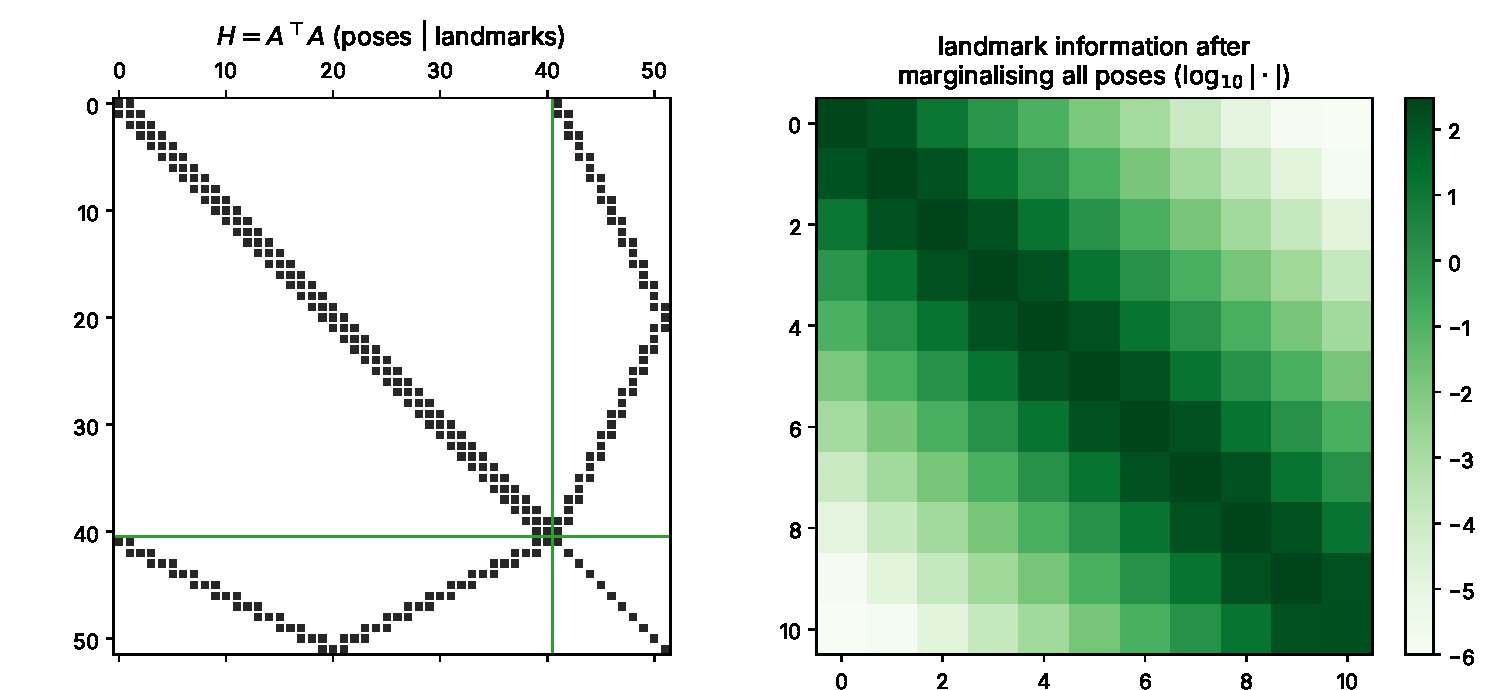
\includegraphics[width=\linewidth]{figures/ch01_sparsity.pdf}
\caption{Left: sparsity of $H=A\T A$ for the 1D problem (poses first,
then landmarks). Right: the landmark information matrix after
marginalising every pose --- dense, as predicted.}
\label{fig:ch1sparsity}
\end{figure}

\begin{figure}[ht]
\centering
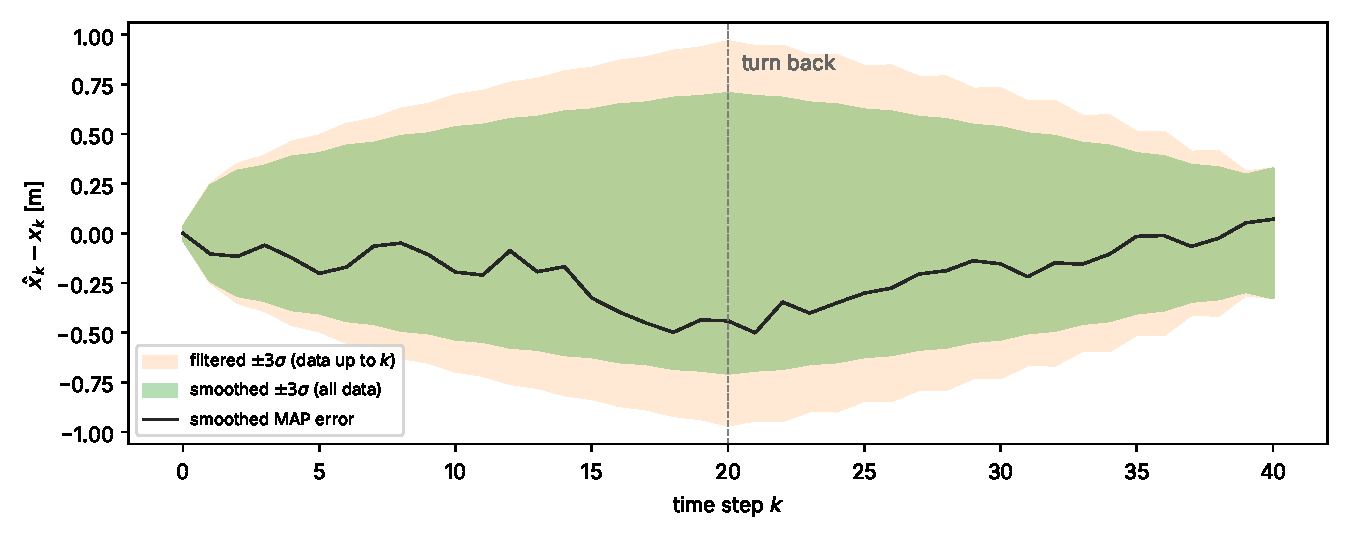
\includegraphics[width=0.9\linewidth]{figures/ch01_trajectory.pdf}
\caption{Filtered (orange) and smoothed (green) $\pm3\sigma$ bands, and
the smoothed MAP error. The filtered uncertainty grows while the robot
meets only new landmarks and shrinks on the way back as it re-observes
known ones: a one-dimensional loop closure. The smoothed uncertainty
depends only on the distance from the start, since every pose benefits
from both legs.}
\label{fig:ch1traj}
\end{figure}

\FloatBarrier
\section*{Exercises}
\addcontentsline{toc}{section}{Exercises}

\begin{enumerate}[label=\textbf{1.\arabic*},ref=1.\arabic*]
\item\label{ex:1tri} In \cref{ex:oned} with no landmarks at all, show
  that $H$ is tridiagonal and positive definite, and that solving it is
  equivalent to running a Kalman filter forwards and a
  Rauch--Tung--Striebel smoother backwards.
\item\label{ex:1gauge} Remove the prior on $x_0$ in \cref{ex:oned}. Show
  that $\vect{1}=(1,\dots,1)\T$ spans the null space of $H$, provided the
  factor graph is connected. Interpret.
\item\label{ex:1marg} In \cref{ex:oned}, marginalise $x_k$ only. Using
  \cref{lem:schur}, write the new factors explicitly and check that they
  connect $x_{k-1}$, $x_{k+1}$ and all landmarks seen at time $k$.
\end{enumerate}

\subsection*{Solutions}

\textbf{1.1.} Without landmarks the only factors are the prior and the
odometry chain, each touching at most two consecutive poses, so by
\cref{prop:sparsity} $H_{ij}=0$ for $|i-j|>1$. Explicitly,
$H=\sigma_0^{-2}\vect{e}_0\vect{e}_0\T+\sigma_u^{-2}\sum_k
(\vect{e}_k-\vect{e}_{k-1})(\vect{e}_k-\vect{e}_{k-1})\T$, a sum of
positive semidefinite terms. If $\btheta\T H\btheta=0$ then $x_0=0$ and
$x_k=x_{k-1}$ for all $k$, so $\btheta=0$: $H\succ0$. Solving a
tridiagonal (more generally block-tridiagonal) system by Gaussian
elimination proceeds in two sweeps. The forward sweep eliminates $x_0$,
then $x_1$, and so on; by \cref{lem:schur} each elimination is a
marginalisation, and the information carried forward to $x_k$ is exactly
the filtered information of $x_k$ given data up to time $k$, i.e.\ the
Kalman filter in information form. The backward substitution recovers
each $x_k$ from $x_{k+1}$, which is the RTS smoother.

\textbf{1.2.} Every remaining row of $A$ has the form
$(\dots,-1,\dots,+1,\dots)/\sigma$, with entries summing to zero, so
$A\vect{1}=\vect{0}$ and $H\vect{1}=\vect{0}$. Conversely, if
$H\btheta=0$ then $\btheta\T H\btheta=\norm{A\btheta}^2=0$, so every
factor forces equal values on its two variables; on a connected graph all
components are equal, and $\btheta\in\operatorname{span}(\vect{1})$.
Interpretation: translating the whole world along the line changes no
relative measurement --- the 1D gauge group is $(\R,+)$, of dimension 1.

\textbf{1.3.} Let $L_k$ be the set of landmarks seen at time $k$. The
blocks of $\Lambda$ touching $x_k$ are $\Lambda_{kk}=2\sigma_u^{-2}+
|L_k|\sigma_z^{-2}$ (if $0<k<K$), $\Lambda_{k,k\pm1}=-\sigma_u^{-2}$ and
$\Lambda_{k,j}=-\sigma_z^{-2}$ for $j\in L_k$. The correction
$\Lambda_{\cdot k}\Lambda_{kk}^{-1}\Lambda_{k\cdot}$ is the outer product
of the column $\vect{\ell}=\Lambda_{\cdot k}$ with itself divided by
$\Lambda_{kk}$, and $\vect{\ell}$ is nonzero exactly on
$\{x_{k-1},x_{k+1}\}\cup L_k$. Hence these variables become pairwise
connected by one new dense factor of information
$\vect{\ell}\vect{\ell}\T/\Lambda_{kk}$, subtracted from the original
blocks.
